\begin{frame}[allowframebreaks]{Multiple Objects}

\begin{figure}
\centering
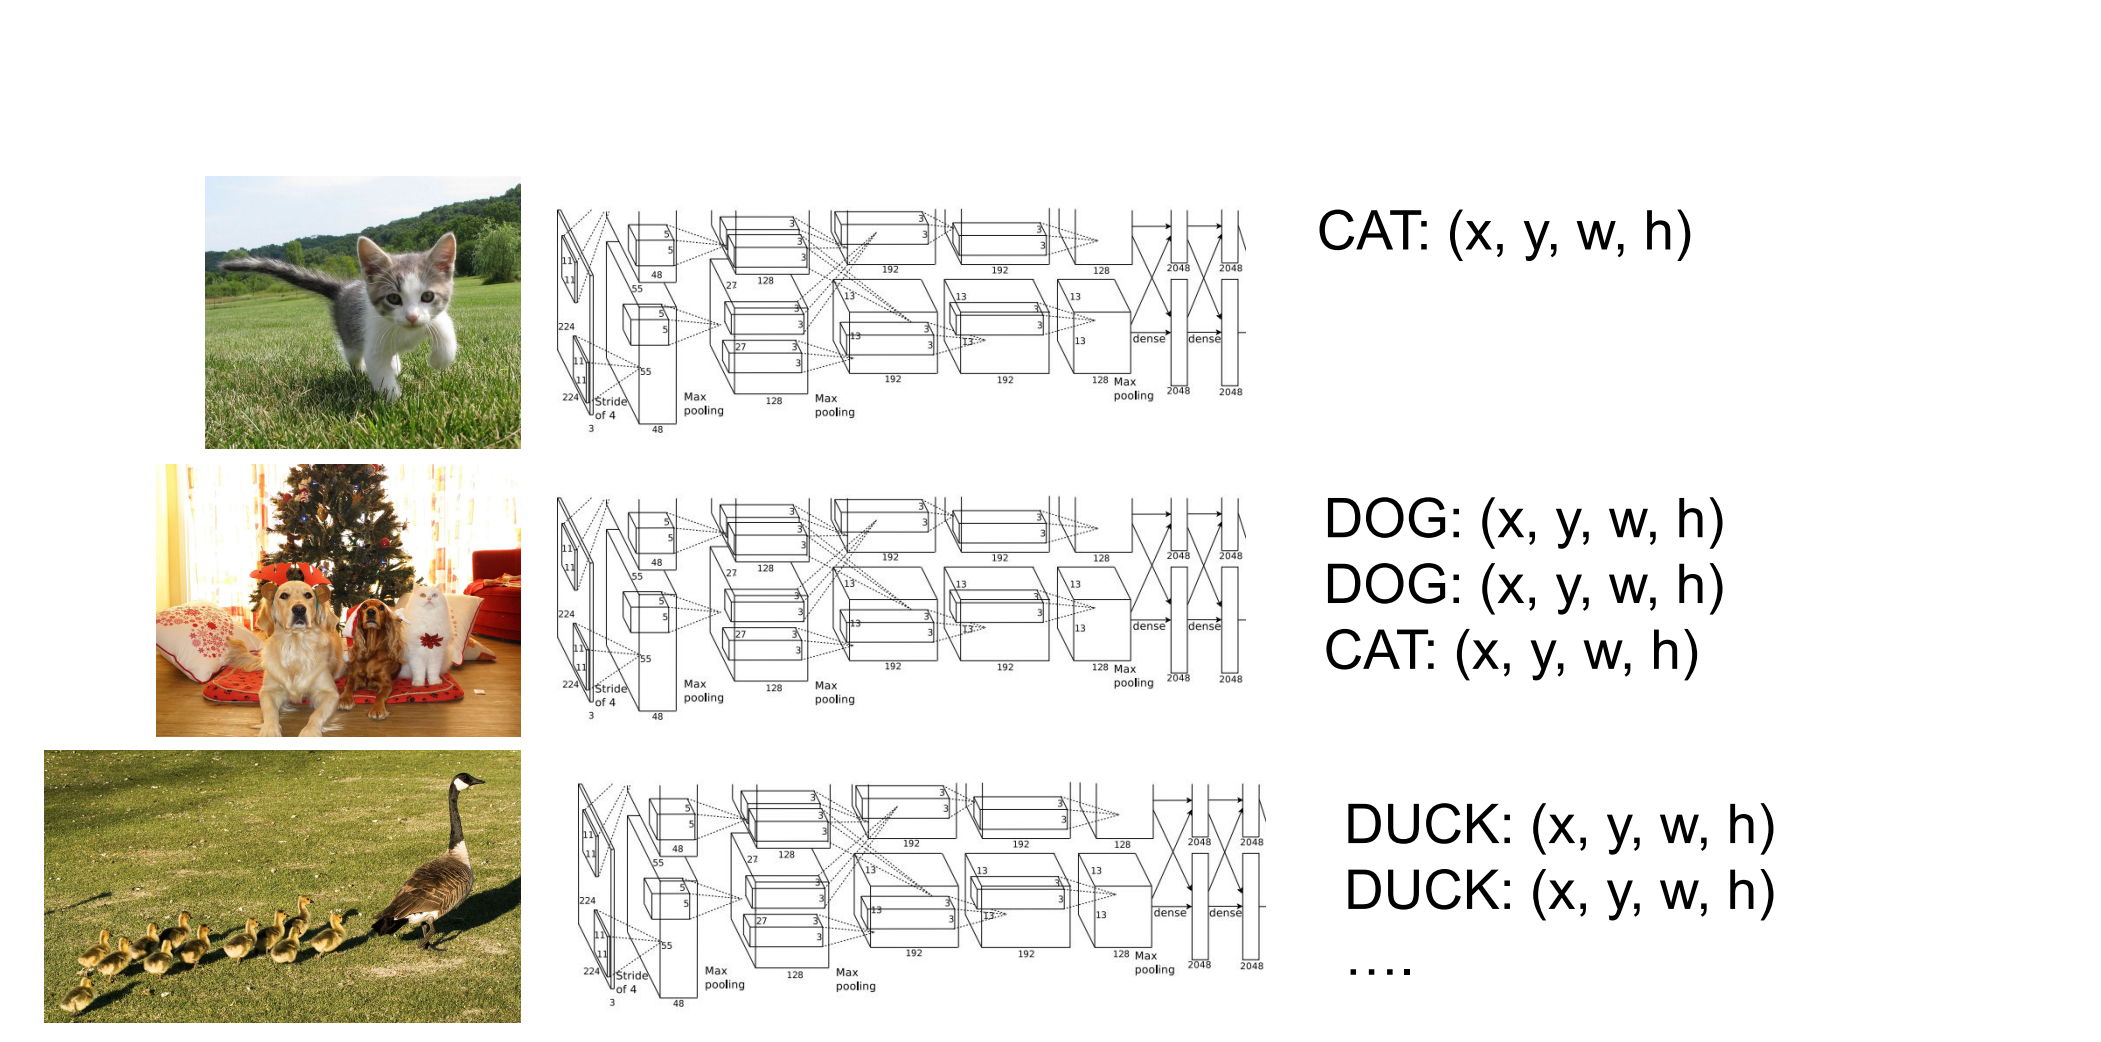
\includegraphics[width=1.0\textwidth,height=1.0\textheight,keepaspectratio]{images/obj-det/object_8.png}
\end{figure}

\framebreak

\begin{figure}
\centering
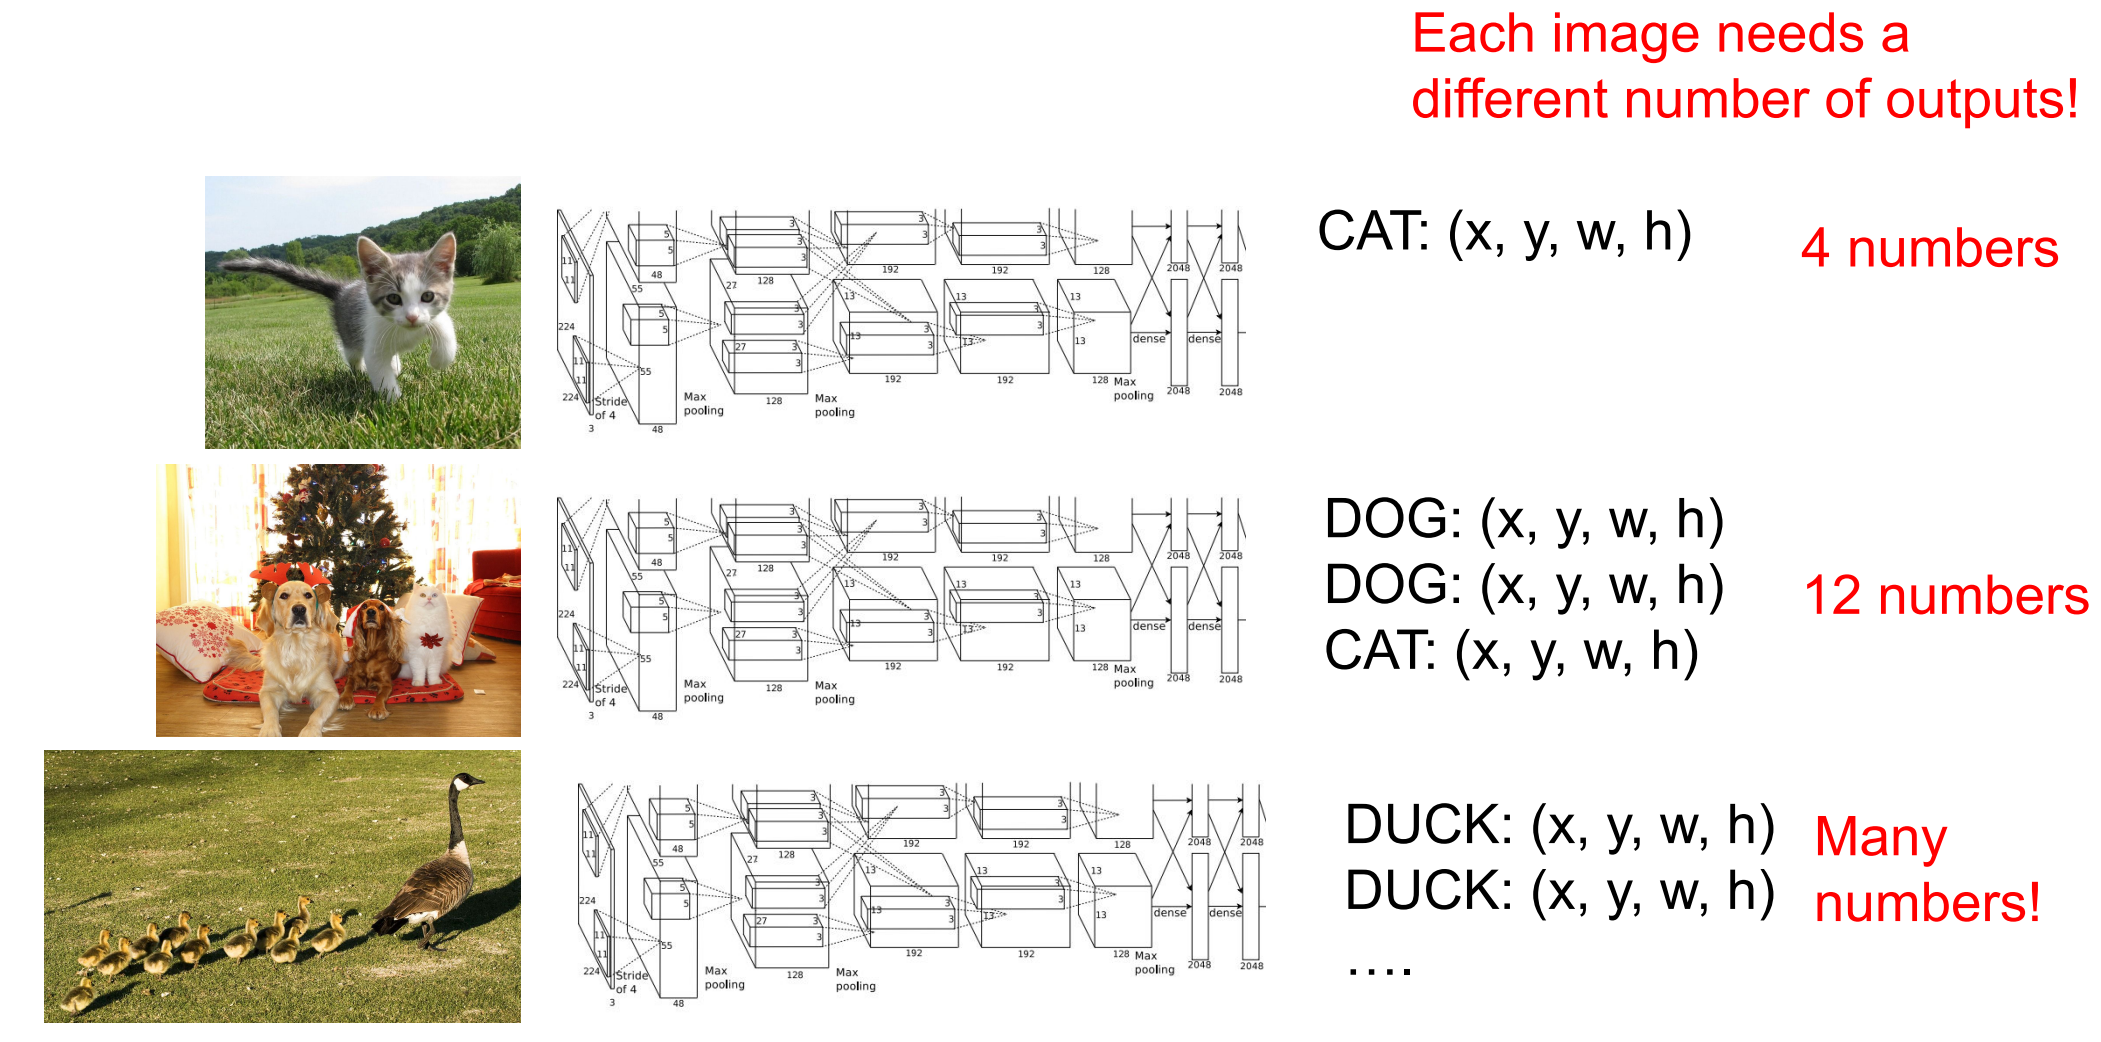
\includegraphics[width=1.0\textwidth,height=1.0\textheight,keepaspectratio]{images/obj-det/object_9.png}
\end{figure}

\end{frame}

\begin{frame}[allowframebreaks]{Detecting Multiple Objects: Sliding Window}

\begin{figure}
\centering
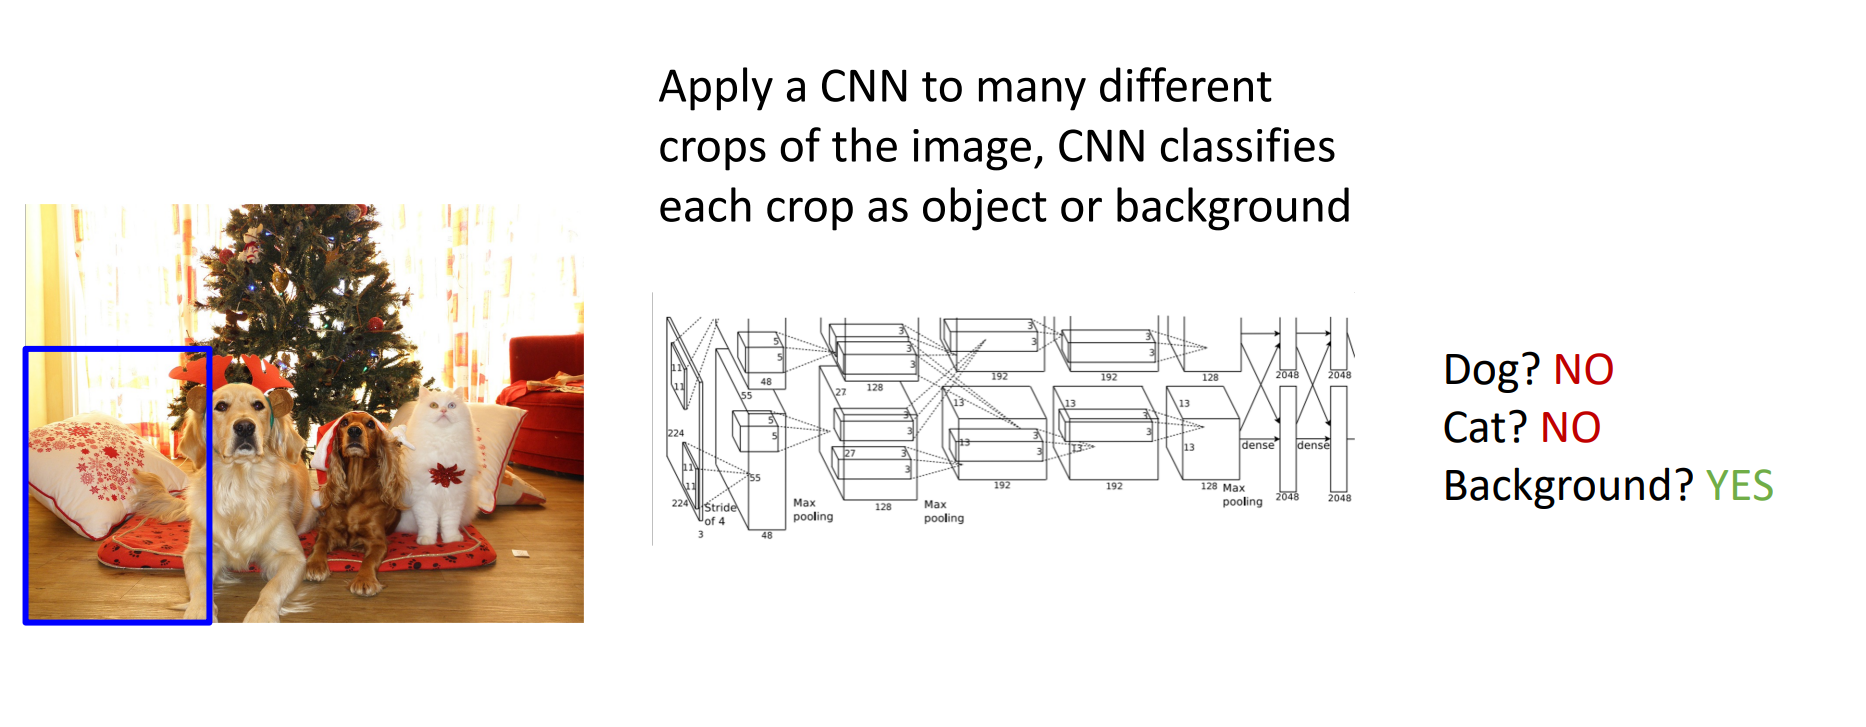
\includegraphics[width=1.0\textwidth,height=1.0\textheight,keepaspectratio]{images/obj-det/object_10.png}
\end{figure}

\framebreak

\begin{figure}
\centering
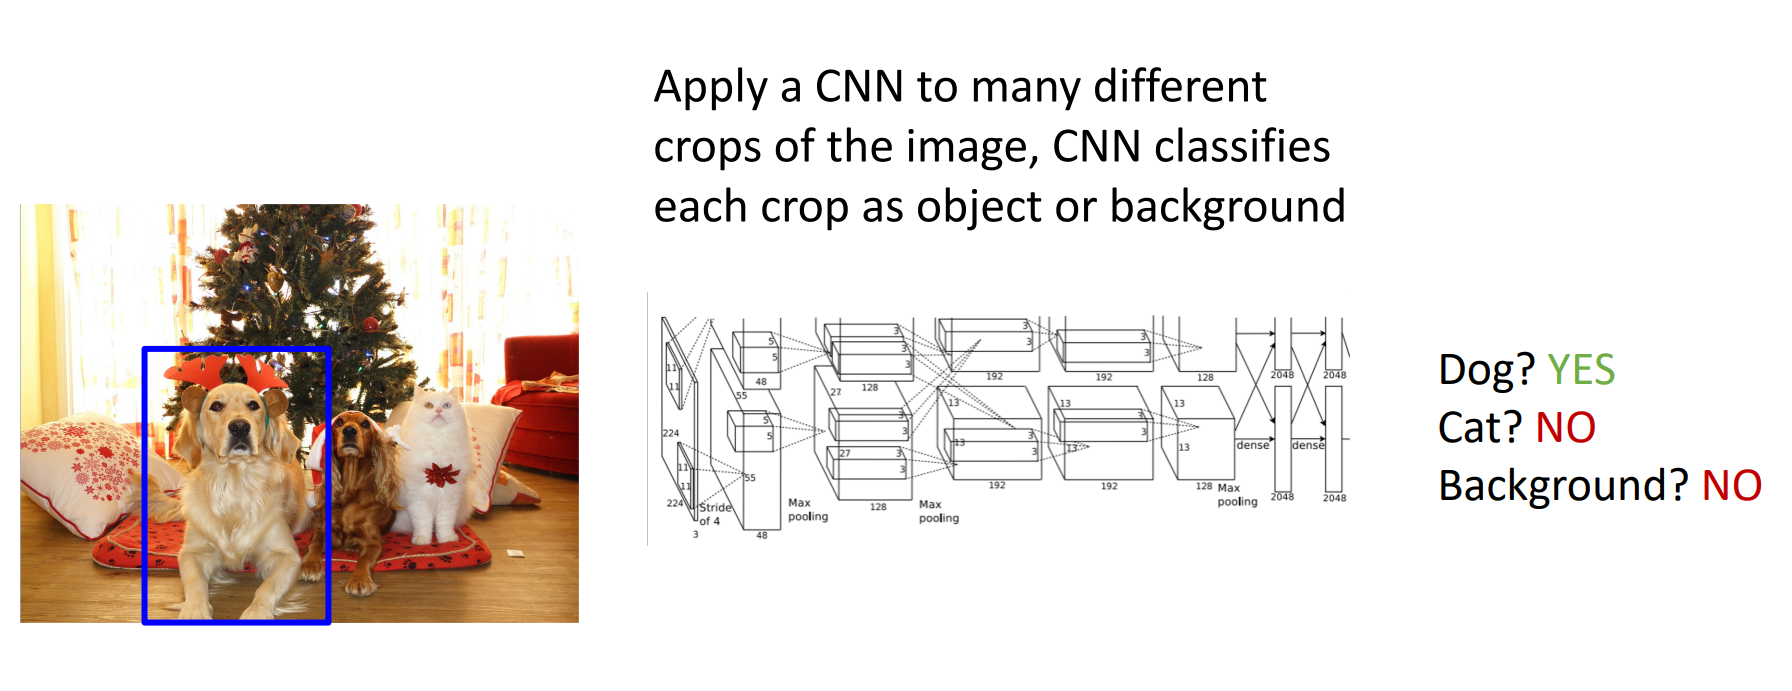
\includegraphics[width=1.0\textwidth,height=1.0\textheight,keepaspectratio]{images/obj-det/object_11.png}
\end{figure}

\framebreak

\begin{figure}
\centering
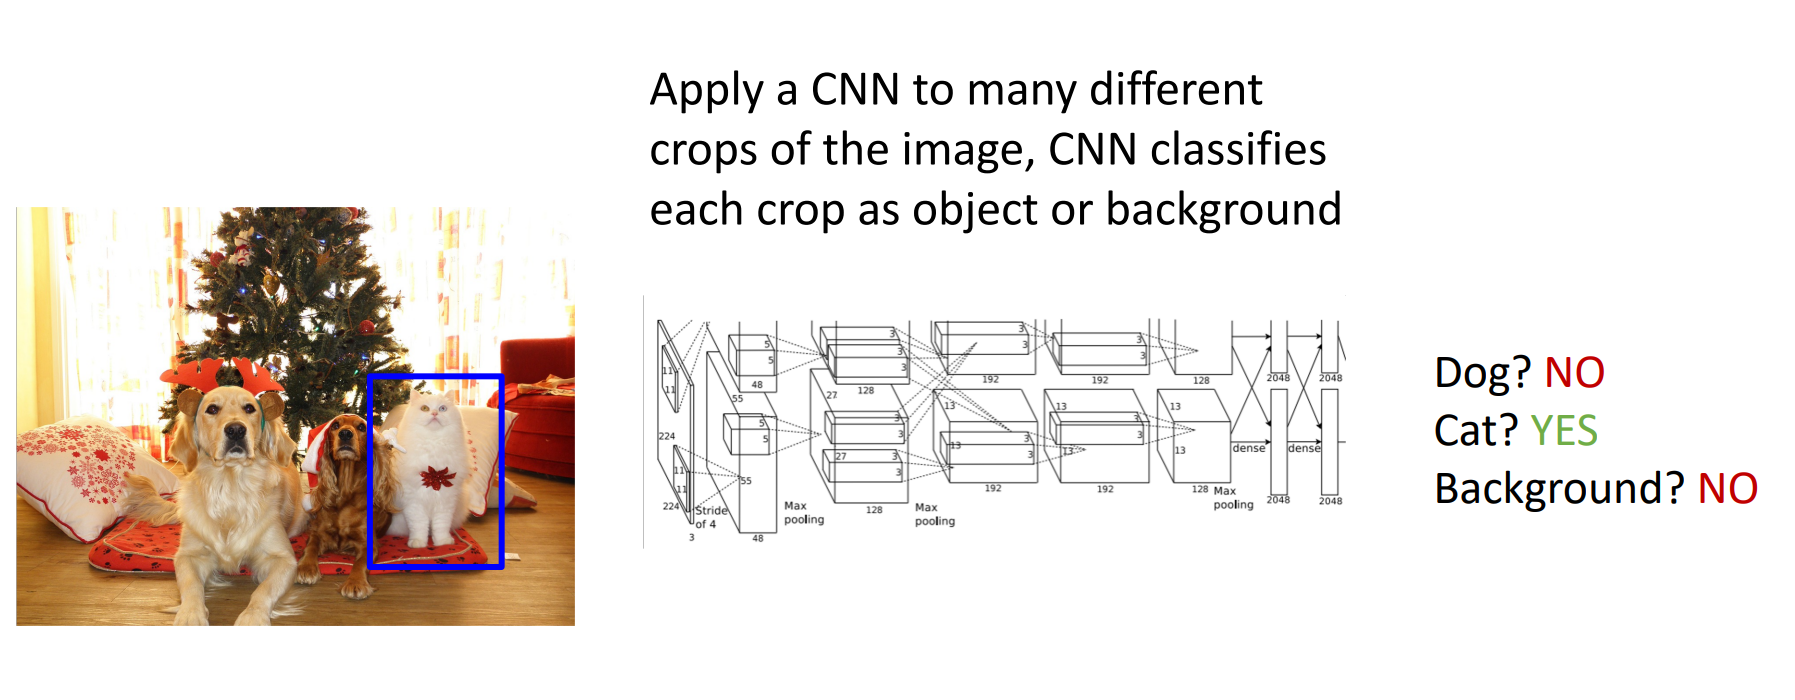
\includegraphics[width=1.0\textwidth,height=1.0\textheight,keepaspectratio]{images/obj-det/object_12.png}
\end{figure}

\framebreak

\begin{figure}
\centering
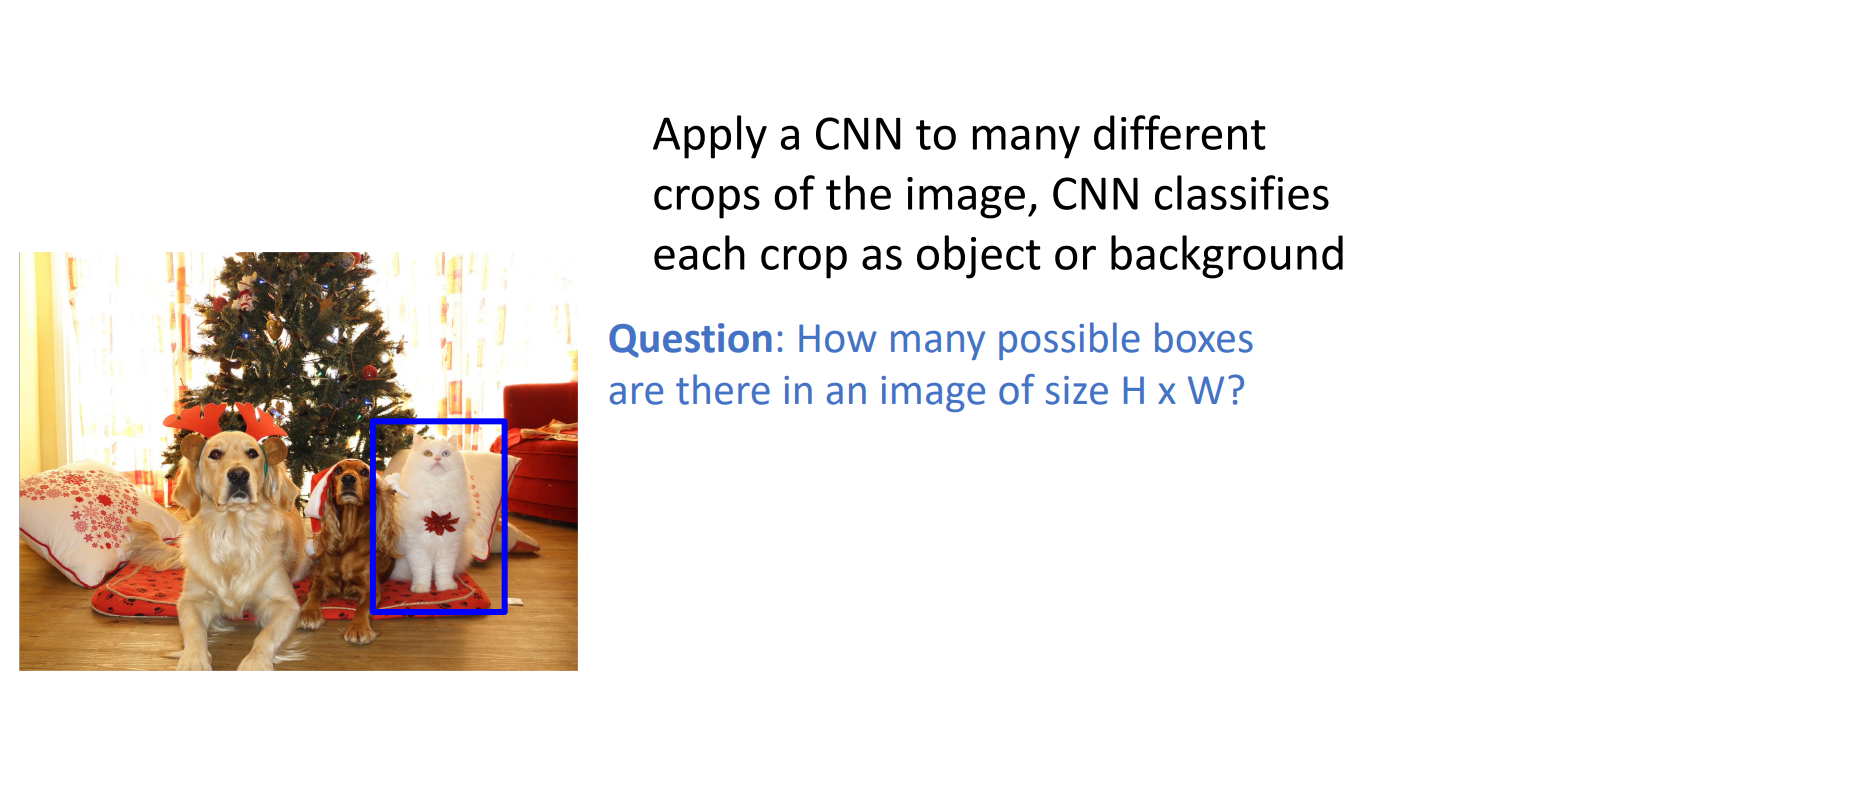
\includegraphics[width=1.0\textwidth,height=1.0\textheight,keepaspectratio]{images/obj-det/object_13.png}
\end{figure}

\framebreak

\begin{figure}
\centering
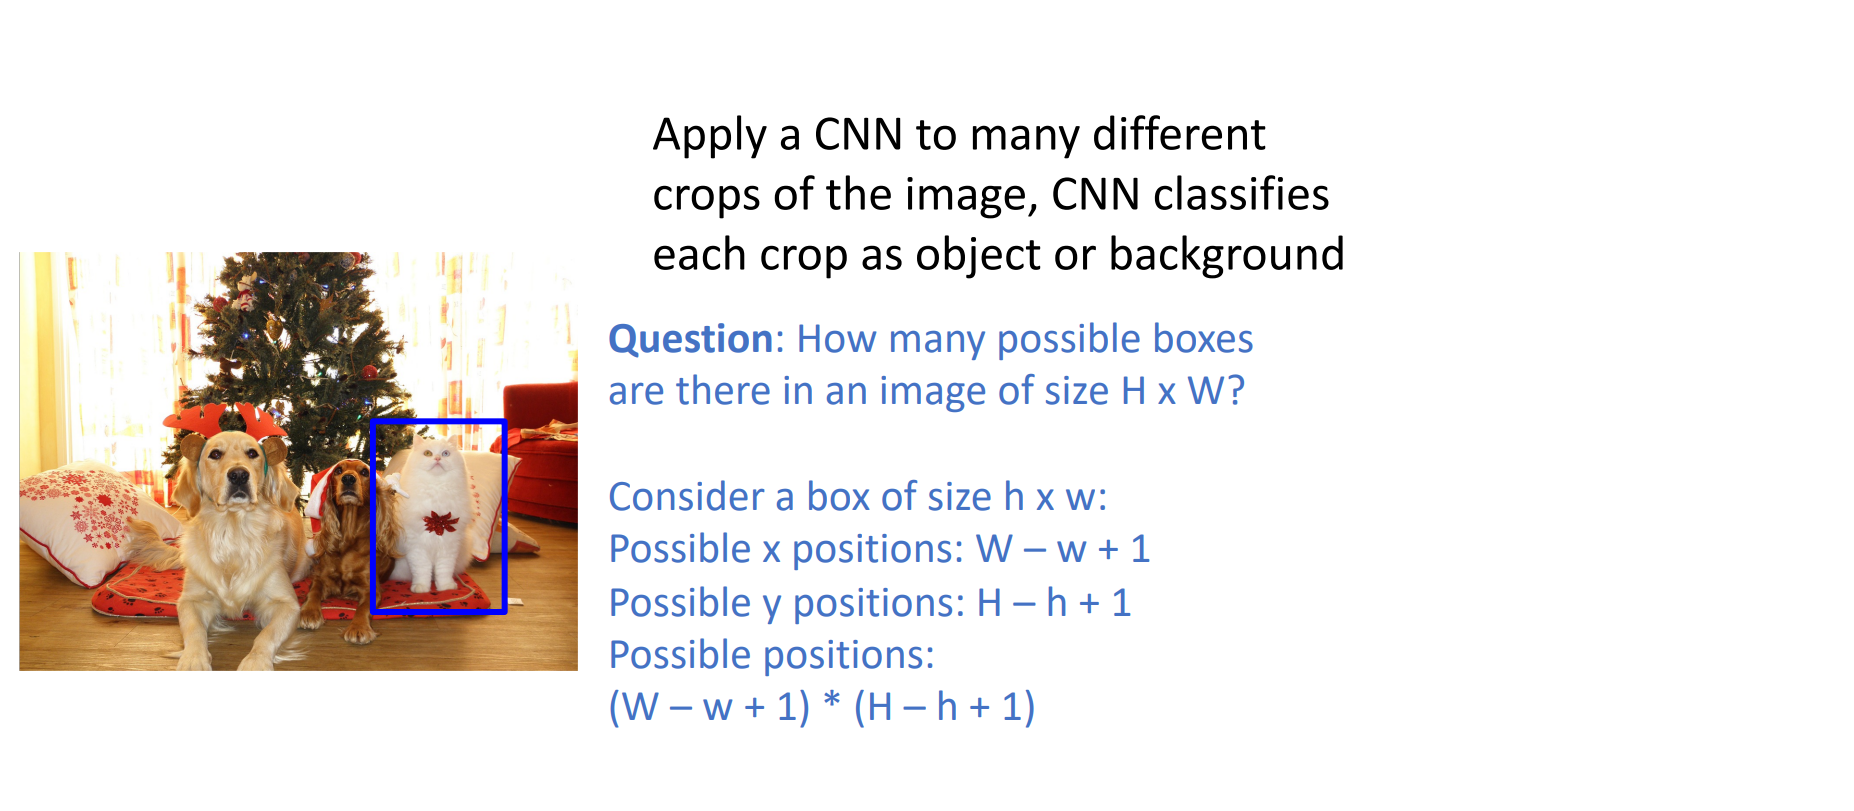
\includegraphics[width=1.0\textwidth,height=1.0\textheight,keepaspectratio]{images/obj-det/object_14.png}
\end{figure}

\framebreak

\begin{figure}
\centering
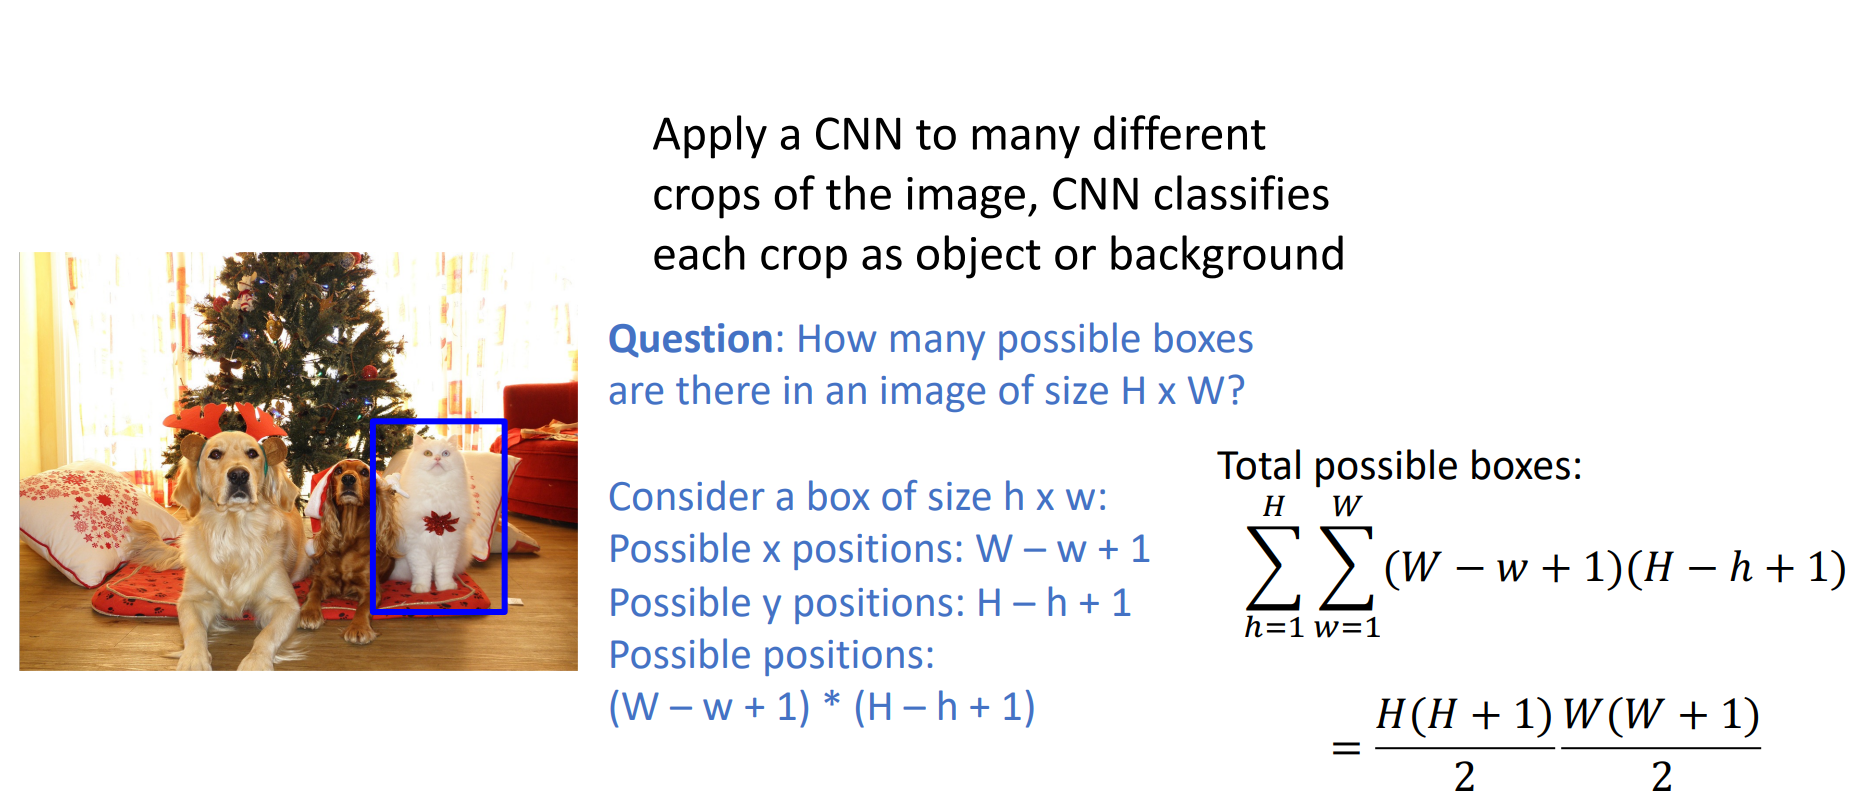
\includegraphics[width=1.0\textwidth,height=1.0\textheight,keepaspectratio]{images/obj-det/object_15.png}
\end{figure}

\framebreak

\begin{figure}
\centering
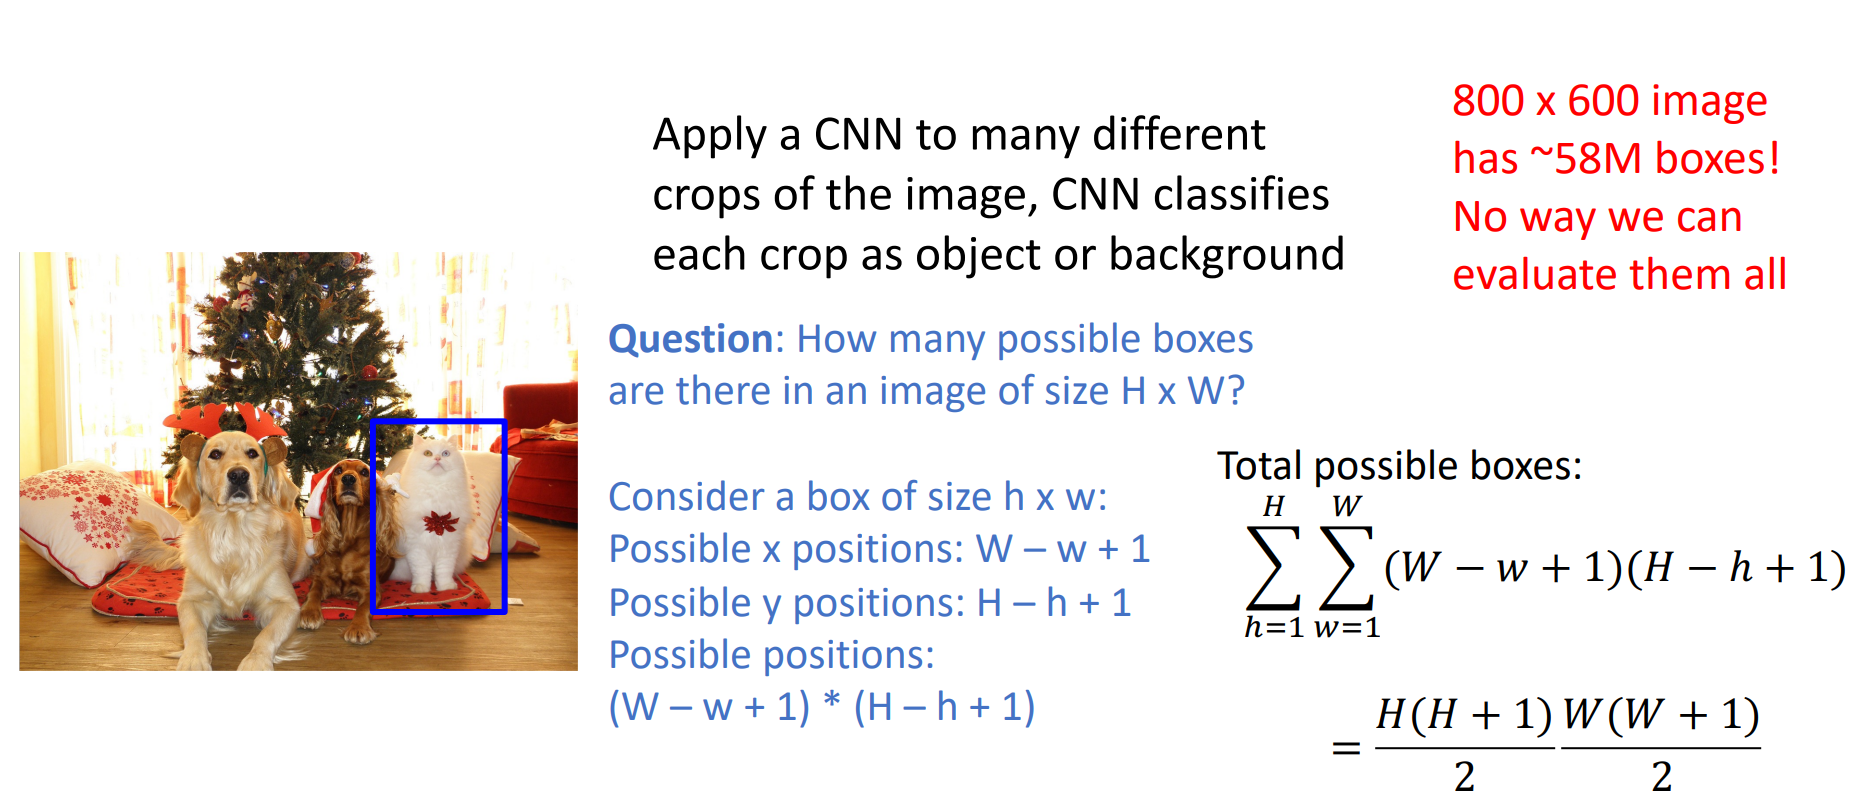
\includegraphics[width=1.0\textwidth,height=1.0\textheight,keepaspectratio]{images/obj-det/object_16.png}
\end{figure}

% Empty Slide Example
\framebreak
\begin{block}{}
    
\end{block}

\end{frame}